% !TEX options=--shell-escape
\documentclass[12pt]{article}
\usepackage[utf8]{inputenc}
\usepackage{lipsum}
\usepackage{afterpage}
\usepackage{mathtools}
\usepackage{xcolor}
\usepackage[12pt]{extsizes}
\usepackage[english,russian]{babel}
\usepackage{cite}
\usepackage{minted}
\usepackage{amsmath, esint, setspace, fancyhdr, amsfonts, bookmark, blindtext}
\usepackage{graphicx}
\usepackage{subfigure}
\usepackage{titlesec}

\graphicspath{{Figures/}}
\DeclareGraphicsExtensions{.pdf,.png,.jpg}
\usemintedstyle{tango}
\definecolor{dhscodebg}{rgb}{0.95,0.95,0.95}


\setlength{\textheight}{8in}
\setlength{\textwidth}{6.6in}
\setlength{\headheight}{0in}
\setlength{\headsep}{0.2in}
\setlength{\topmargin}{0in}
\setlength{\oddsidemargin}{0in}
\setlength{\evensidemargin}{0in}
\setlength{\parindent}{.3in}

\doublespacing
\renewcommand{\baselinestretch}{1.4} 
\newcommand{\RNumb}[1]{\uppercase\expandafter{\romannumeral #1\relax}}

\begin{document}
\begin{titlepage}

\begin{center}
Санкт-Петербургский политехнический университет Петра Великого\\
Институт прикладной математики и механики\\
Кафедра прикладной математики\\
\end{center}


\vspace{2.5cm}

\begin{center}
{\large {\bfseries СВОДНЫЙ ОТЧЕТ}}\\

\bigskip \bfseries{Тема:} {\bfseries \emph{Многомерные распределения.\\ Оценки характеристик распределений}}
\end{center}

\vspace{1.5cm}

\begin{flushleft}
Направление: 01.03.02 Прикладная математика и информатика

\vspace{1.5cm}

Выполнил студент гр. 33631/4 \hfill{Камалетдинова Ю.} \\ 

\vspace{0.5cm} Преподаватель \hfill{Баженов А.}
\vspace{1cm}

\end{flushleft}

\vspace{2.7cm}

\begin{center}
Санкт-Петербург\\
2019
\end{center}

\end{titlepage}

\newcommand{\threeimage}[4]{
\begin{figure}[h!]  
    \centering 
    \subfigure[]{
        \includegraphics[width=0.3\linewidth, height=0.25\linewidth]{#1} 
        \label{fig:f_ #1} }  
        %\hspace{4ex}
    \subfigure[]{
    \includegraphics[width=0.3\linewidth, height=0.25\linewidth]{#2} 
    \label{fig:f_ #2} }
   % \hspace{4ex}
    \subfigure[]{ 
        \includegraphics[width=0.3\linewidth, height=0.25\linewidth]{#3} 
        \label{fig:f_ #3} }  
    \caption{Выборки из #4 объемом: 
    \subref{fig:f_ #1} 20; 
    \subref{fig:f_ #2} 60; 
    \subref{fig:f_ #3} 100} 
    \label{fig:f_ #1#2#3}
\end{figure}}

\newcommand{\triplethreeimage}[4]{
\begin{figure}[h!]  
    \centering 
    \subfigure[]{
        \includegraphics[width=.83\linewidth, height=.3\linewidth]{#1} 
        \label{fig:f_ #1} }\\  
    %\hspace{4ex}
    \subfigure[]{
        \includegraphics[width=.83\linewidth, height=.3\linewidth]{#2} 
        \label{fig:f_ #2} }\\
    %\hspace{4ex}
    \subfigure[]{ 
        \includegraphics[width=.83\linewidth, height=.3\linewidth]{#2} 
        \label{fig:f_ #3} }  
    \caption{Для выборок из #4 объемом: 
    \subref{fig:f_ #1} 20; 
    \subref{fig:f_ #2} 60; 
    \subref{fig:f_ #3} 100} 
    \label{fig:f_ #1#2#3}
\end{figure}}


\tableofcontents
\addtocontents{toc}{~\hfill\par}
\vfill ~
\setcounter{section}{0}

%%%%%%%%%%%%%%%%%%%%%%%%%%%%%%%%%%%%%%%%%%

\newpage 
\section*{Постановка задачи}
\addcontentsline{toc}{section}{Постановка задачи}

\indent{\indent В данной группе лабораторных работ рассматриваются многомерные распределения и методы оценки характеристик распределений. Запишем постановки задач}
\begin{itemize}
    \item { Cгенерировать двумерные выборки $x_n = (x_1, \ldots, x_n), \; y_n = (y_1, \ldots, y_n)$ размерами $n = 20,\;60,\;100$ из нормального двумерного распределения. Коэффициенты корреляции взять равными $\rho = 0, \; 0.5, \; 0.9$. Формула для плотности распределения приведена ниже 
        \begin{equation}
            \label{dist_5:1}
            N(x, y, 0, 0, 1, 1, \rho) = \frac{1}{2\pi \sqrt{1-\rho^2}}exp\left\{-\frac{1}{2(1-\rho^2)}(x^2 - 2\rho xy + y^2)\right\}
        \end{equation}
    \indent Каждая выборка генерируется $N = 1000$ раз, и для каждоый выборки вычисляются среднее значение, среднее значение квадрата и дисперсия следующих коэффициентов
        \begin{equation}
            \label{coeff_5:1}
            r_{p} = \frac{\displaystyle \sum_{i=1}^{n}{(x_i - \overline{x})(y_i - \overline{y})}}{\sqrt{\displaystyle{\sum_{i=1}^{n}{(x_i - \overline{x})^2 \sum_{i=1}^{n}(y_i - \overline{y})^2}}}} = \frac{cov(x, y)}{\sqrt{\sigma^2_x \sigma^2_y}} \text{ –– коэффициент корреляции Пирсона,}
        \end{equation}
    \indent где $\overline{x}, \; \overline{y}$ –– выборочные средние $x_n, \; y_n$, $\sigma^2_x, \; \sigma^2_y$ –– выборочные дисперсии
    
    \begin{equation}
        \label{coeff_5:2}
        r_s = \rho_{rg_x, rg_y} = \frac{cov(rg_x, rg_y)}{\sqrt{\sigma^2_x \sigma^2_y}} = 1 - \frac{6 \displaystyle \sum_{i=1}^{n}{d^2_i}}{n(n^2-1)} \text{ –– коэффициент корреляции Спирмена,}
    \end{equation}
    \indent где $rg_x, \; rg_y$ –– ранговые переменные, $d_i = rg(x_i) - rg(y_i)$ –– разность двух рангов наблюдений. Формула для рассчета из источника \cite{ms_2}
    
    \begin{equation}
        \label{coeff_5:3}
        r_q = \frac{(n_{\RNumb{1}} + n_{\RNumb{3}}) - (n_{\RNumb{2}} + n_{\RNumb{4}})}{n} \text{ –– квадрантный коэффициент корреляции,}
    \end{equation}
    \indent где $n_i, \; i = \RNumb{1},\; \RNumb{2},\; \RNumb{3},\; \RNumb{4}$ –– число наблюдений, попавших в $i$ - ый квадрант на плоскости
    
    \indent Приведем формулы для вычисления выборочного среднего, квадрата выборочного среднего и выборочной дисперсии в двумерном случае
    \begin{equation}
        \label{char_5:1}
        \overline{x}_k = \frac{1}{n}\sum_{i=1}^{n}{x_{i_k}}, \;\; k = 1, \; 2
    \end{equation}
    
    \begin{equation}
        \label{char_5:2}
        \overline{x}^2_k = \frac{1}{n}\sum_{i=1}^{n}{x^2_{i_k}}, \;\; k = 1, \; 2
    \end{equation}
    
    \begin{equation}
        \label{char_5:3}
        \overline{\sigma}^2_k = \frac{1}{n}\sum_{i=1}^{n}{(x_{i_k}-\overline{x}_k)^2}, \;\; k = 1, \; 2
    \end{equation}
    
    \indent Требуется повторить вычисления характеристик \eqref{char_5:1}, \eqref{char_5:2}, \eqref{char_5:3}  корреляционных коэффициентов \eqref{coeff_5:1}, \eqref{coeff_5:2}, \eqref{coeff_5:3} для смеси нормальных распределений
    
    \begin{equation}
        \label{dist_5:2}
        f(x, y) = 0.9 N(x, y, 0, 0, 1, 1, 0.9) + 0.1 N(x, y, 0, 0, 10, 10, -0.9)
    \end{equation}
    \indent Полученные выборки необходимо изобразить на плоскости и изобразить эллипс равновероятности }
    \item {Найти оценки коэффициентов линейной регрессии $y_i = a + bx_i + e_i$, используя $n = 20$ точек на отрезке $[-1.8; 2]$ с равномерным шагом равным 0.2. Ошибку $e_i$ считать нормально распределенной с параметрами (0, 1). В качестве эталонной зависимости взять функцию
\begin{equation}
    \label{eq_6:1}
    y_i = 2 + 2x_i + e_i 
\end{equation}
\indent При построении оценок коэффициентов использовать два критерия: критерий наименьших квадратов и критерий наименьших модулей. Требуется проделать описанную работу для выборки, у которой в значения $y_1$ и $y_{20}$ вносятся возмущения $10$ и $-10$.}
    \item {Сгенерировать выборку объемом $n = 100$ элементов для нормального распределения $N(x; 0, 1)$ и оценить по ней параметры $\mu$ и $\sigma$ нормального распределения методом максимального правдоподобия. В качестве основной гипотезы $H_0$ будем считать, что сгенерированное распределение имеет вид $N(x; \hat{\mu}, \hat{\sigma})$. Проверить гипотезу, используя критерий согласия $\chi^2$. В качестве уровня значимости взять $\alpha = 0.05$. Привести таблицу вычислений $\chi^2$.}
    \item {Сгенерировать выборки объемами $n = 20, \; 100$ элементов для нормального распределения $N(x; 0, 1)$, затем для параметров положения и масштаба построить асимптотически нормальные интервальные оценки на основе точечных оценок метода максимального правдоподобия. Также необходимо оценить параметры распределения на основе статистик $\chi^2$ и Стьюдента. В качестве параметра надежности взять $\gamma = 0.95$.}
\end{itemize}

%%%%%%%%%%%%%%%%%%%%%%%%%%%%%%%%%%%%%%%%%%

\section*{Описание алгоритма}
\addcontentsline{toc}{section}{Описание алгоритма}
\subsection*{Метод наименьших квадратов}

\indent{\indent Введем обозначение для уравнения прямой, полученного по тому или иному критерию рассогласованности отклика и регрессионной модели}
\begin{equation}
    \label{eq_6:2}
    \hat y_i = \hat a + \hat bx_i ,
\end{equation}
где $\hat{a}, \hat{b}$ –– оценки параметров $a, b$

\indent{Запишем минимизируемое выражение для случая критерия наименьших квадратов (МНК)}
\begin{equation}
    \label{crit_6:1}
    Q(a, b) = \sum_{i=1}^{n}\epsilon^2 = \sum_{i=1}^{n}{(y_i - a - bx_i)^2} \rightarrow \underset{a, b} min
\end{equation}

\indent{Опустим запись необходимых условий экстремума и доказательства минимальности функции \eqref{crit_6:1} в стационарной точке, описанных в \cite{ms_4}, и приведем МНК-оценки коэффициентов}

\begin{equation}
    \label{coeff_6:1}
    \hat b = \frac{\overline{xy} - \overline{x} \cdot \overline {y}}{\overline{x^2} - (\overline{x})^2}
\end{equation}

\begin{equation}
    \label{coeff_6:2}
    \hat a = \overline{y} - \overline{x} \hat b,
\end{equation}

где $\overline{x}, \; \overline{x^2}, \; \overline{y}, \; \overline{xy}$ –– выборочные первые и вторые начальные моменты

\subsection*{Метод наименьших модулей}

\indent{\indent Одной из альтернатив МНК является метод наименьших модулей (МНМ)}
\begin{equation}
    \label{crit_6:2}
    A(a, b) = \sum_{i=1}^{n}{|y_i - a - bx_i|} \rightarrow \underset{a, b} min
\end{equation}

\indent{Запишем выражения для оценок \eqref{coeff_6:1}, \eqref{coeff_6:2} в другом виде}

\begin{equation}
    \label{coeff_6:3}
    \hat b = \frac{\overline{xy} - \overline{x} \cdot \overline {y}}{\overline{x^2} - (\overline{x})^2} = \frac{k_{xy}}{s_xs_y} = \frac{k_{xy}}{s^2_y} \frac{s_y}{s_x} = r_{xy} \frac{s_y}{s_x}
\end{equation}

\begin{equation}
    \label{coeff_6:4}
    \hat a = \overline{y} - \overline{x} \hat b,
\end{equation}

\indent{В формулах \eqref{coeff_6:3}, \eqref{coeff_6:4} заменим выборочные средние $\overline{x}, \; \overline{y}$ на выборочные медианы $med \; x, \; med \; y$, а среднеквадратические отклонения $s_x, \; s_y$ на интерквартильные широты $IQR_x, \; IQR_y$;  выборочный коэффициент корреляции $r_{xy}$ –– на знаковый коэффициент корреляции $r_Q$ }

\begin{equation}
    \label{coeff_6:5}
    \hat b_R = r_q \frac{IQR_y}{IQR_x},
\end{equation}

\begin{equation}
    \label{coeff_6:6}
    \hat a_R = med \; y - \hat b_R \; med \; x,
\end{equation}

\begin{equation}
    \label{coeff_6:7}
    r_Q = \frac{1}{n} \sum_{i=1}^{n}{sign(x_i - med \; x) \; sign(y_i - med \; y)}
\end{equation}

\begin{equation}
    \label{eq_6:3}
    sign \; z = 
    \begin{cases}
    \;\;\;1, \; z > 0 \\
    \;\;\;0, \; z = 0 \\
    -1, \;z < 0
    \end{cases}
\end{equation}

\indent{Формулы \eqref{coeff_6:3}, \eqref{coeff_6:4}, \eqref{coeff_6:5}, \eqref{coeff_6:6}, \eqref{coeff_6:7}, \eqref{eq_6:3} указаны в учебнике \cite{ms_4}. Уравнение регрессии примет вид}

\begin{equation}
    \label{eq_6:4}
    y = \hat a_R + \hat b_R x
\end{equation}

\subsection*{Метод максимального правдоподобия}
\indent{\indent Пусть $x_1, \ldots, x_n$ –– случайная выборка из распределения с плотностью вероятности $f(x; \theta)$. Функцией правдоподобия (ФП) назовем совместную плотность вероятности независимых случайных величин $x_1, \ldots, x_n$, рассматриваемую как функцию неизвестного параметра $\theta$}

\begin{equation}
	L(x_1, \ldots, x_n; \theta) = f(x_1; \theta)f(x_2; \theta)\ldots f(x_n; \theta)
	\label{eq_7:1}
\end{equation}

\indent{ Оценкой максимального правдоподобия $\hat\theta_{\text{МП}}$ будем называть такое значение, для которого из множества допустимых значений параметра $\theta$ ФП имеет наибольшее значение при заданных $x_1, \ldots, x_n$}

\begin{equation}
	\hat\theta_{\text{МП}} = arg \; max \; L(x_1, \ldots, x_n; \theta)
	\label{eq_7:2}
\end{equation}

\indent{ Если функция правдоподобия дважды дифференцируема, ее стационарные значения задаются корнями уравнения}

\begin{equation}
	\frac{\partial{L(x_1, \ldots, x_n; \theta)}}{\partial{\theta}} = 0
	\label{eq_7:3}
\end{equation}

Запишем условие локального максимума $\overline{\theta}$

\begin{equation}
	\frac{\partial^2 L}{\partial \theta^2} (x_1, \ldots, x_n; \overline{\theta}) 
	< 0
	\label{eq_7:4}
\end{equation}
Наибольший локальный максимум будет являться решением задачи \eqref{eq_7:2}. 

\indent{ Мы будем искать максимум логарифма функции правдоподобия в виду того, что он имеет максимум в одной точке с функцией правдоподобия}

\begin{equation}
	\frac{\partial \ln L}{\partial \theta} \text{, если $L > 0$,}
	\label{eq_7:5}
\end{equation}
и будем решать уравнение правдоподобия

\begin{equation}
    \frac{\partial \ln  L}{\partial \theta} = 0
    \label{eq_7:6}
\end{equation}

\indent{ Для проверки гипотезы о характере распределения воспользуемся критерием $\chi^2$ для случая, когда параметры распределения известны. Пусть $H_0$ –– гипотеза о генеральном законе распределения, $H_1$ –– гипотеза о справедливости одного из конкурирующих законов распределений. Разобьем генеральную совокупность на $k$ непересекающихся подмножеств $\Delta_1, \ldots, \Delta_k$ при условиях}

\begin{equation}
    p_i = P(X \in \Delta_i), \; i = \overline{1,k}\;; \;\; \sum_{i=1}^{k} p_i = 1
    \label{cond_7:1}
\end{equation}

\indent{ Положим $n_i$ –– частота попадания выборочного элемента в подмножество $\Delta_i$. За меру отклонения выборочного распределения от гипотетического примем величину}

\begin{equation}
    Z = \sum_{i=1}^{k}c_i \left(\frac{n_i}{n} - p_i\right)^2,
    \label{eq_7:7}
\end{equation}
где $\frac{n_i}{n}$ –– относительные частоты, $c_i$ –– некие положительные числа (веса). В качестве весов К. Пирсоном были взяты числа $c_i = \frac{n}{p_i}$. Получаем статистику критерия хи-квадрат К. Пирсона

\begin{equation}
    \chi^2 = \sum_{i=1}^{k}\frac{n}{p_i} \left(\frac{n_i}{p} - p_i\right)^2 = \sum_{i=1}^{k}\frac{(n_i - np_i)^2}{np_i}
    \label{eq_7:8}
\end{equation}

\indent{ По теореме К. Пирсона из пособия \cite{ms_4} статиcтика критерия $\chi^2$ асимптотически распределена по закону $\chi^2$ с $k - 1$ степенями свободы}


\indent{ Формулы \eqref{eq_7:1} –– \eqref{eq_7:8} и определения взяты из источника \cite{ms_4}}

\subsection*{Оценка на основе статистик Стьюдента и хи-квадрат}

\indent{\indent Пусть $x_1, \ldots, x_n$ –– заданная выборка из нормального распределения $N(x; \mu, \sigma)$, по которой требуется оценить параметры $\mu$, $\sigma$, генерального распределения. Построим на ее основе выборочные среднее $\overline{x}$ и среднее квадратическое отклонение $s$. Параметры распределения $\mu, \; \sigma$ не известны. В источнике \cite{ms_4} показано, что статистика Стьюдента}

\begin{equation}
	T = \sqrt{n - 1}\;\frac{\overline{x} - \mu}{s}
	\label{eq_8:1}
\end{equation}
распределена по закону Стьюдента с $n - 1$ степенями свободы. Пусть $f_T(x)$ –– плотность вероятности данного распределения. Тогда

\begin{equation}
    \begin{aligned}        
        P(-x < \sqrt{n - 1} \; \frac{\overline{x} - \mu}{s} < x) = P(-x < \sqrt{n - 1} \; \frac{\mu - \overline{x}}{s} < x) = \\
        =\int_{-x}^{x}f_T(t)dt = 2 F_T(x) - 1 \; ,
        \label{eq_8:2}
\end{aligned}
\end{equation}
где $F_T(t)$ –– функция распределения Стьюдента с $n - 1$ степенями свободы.
\indent{ Положим $2 F_T(x) - 1 = 1 - \alpha$, где $\alpha$ –– выбранный уровень значимости. Тогда $F_T(x) = 1 - {\alpha}/{2}$. Положим $t_{1- {\alpha}/{2}}(n - 1)$ –– квантиль распределения Стьюдента с $n - 1$ степенями свободы и уровнем значимости $1 - {\alpha}/{2}$. Из \eqref{eq_8:1}, \eqref{eq_8:2} получаем}


\begin{equation}
        P\left(\overline{x} - \frac{s t_{1 - {\alpha}/{2}}(n-1)}{\sqrt{n - 1}} < \mu < \overline{x} + \frac{s t_{1 - {\alpha}/{2}}(n-1)}{\sqrt{n - 1}}\right) = 1 - \alpha \; ,
	\label{eq_8:3}
\end{equation}
что дает доверительный интервал для $\mu$ с вероятностью $\gamma = 1 - \alpha$

\indent{ Для поиска оценки параметра $\sigma$ воспользуемся источником \cite{ms_4}, где показано, что случайная величина $n {s^2}/{\sigma^2}$ распределена по закону $\chi^2$ с $n - 1$ степенями свободы. }
\indent{ Найдем квантили $\chi_{{\alpha}/{2}}^2(n - 1), \;\; \chi_{1 - {\alpha}/{2}}^2(n - 1)$ и приведем выражение для доверительного интервала для $\sigma$ с доверительной вероятностью $\gamma = 1 - \alpha$}

\begin{equation}
    P\left(\frac{s \sqrt{n}}{\sqrt{\chi_{1 - {\alpha}/{2}}^2(n - 1)}} < \sigma < \frac{s \sqrt{n}}{\sqrt{\chi_{ {\alpha}/{2}}^2(n - 1)}} \right) = 1 - \alpha
    \label{eq_8:4}
\end{equation}

\subsection*{Асимптотический подход при построении оценок}

\indent{\indent Данный метод оценивания параметров применяется в случае неизвестности закона распределения, или когда он не является нормальным. Асимптотический метод построения доверительных интервалов основан на центральный предельной теореме.}

\indent{ Пусть $\overline{x}$ –– выборочное среднее из выборки большого объема $n$ независимых одинаково распределенных случайных величин. Тогда в силу центральной предельной теоремы случайная величина $(\overline{x} - M\overline{x})/ \sqrt{D\overline{x}} = \sqrt{n}(\overline{x} - \mu)/ \sigma$ распределена приблизительно нормально с параметрами 0, 1. Из данных рассуждений получим выражение для доверительного интервала для $\mu$ с доверительной вероятностью $\gamma = 1 - \alpha$}
\begin{equation}
    P\left(\overline{x} - \frac{su_{1 - \alpha / 2}}{\sqrt{n}} < \mu < \overline{x} + \frac{su_{1 - \alpha / 2}}{\sqrt{n}} \right) \approx \gamma \; , 
    \label{eq_8:5}
\end{equation}
где $u_{1 - \alpha / 2}$ –– квантиль распределения $N(0, 1)$ порядка $1 - \alpha / 2$

\indent{ Приведем выражение для доверительного интервала для $\sigma$ с доверительной вероятностью $\gamma = 1 - \alpha$}
\begin{equation}
    s\left(1 - 0.5U\right) < \sigma < s\left(1 + 0.5U\right) \; , 
    \label{eq_8:6}
\end{equation}
где $U = u_{1 - \alpha / 2} \sqrt{(e + 2) / n}$;  $e$ –– выборочный эксцесс; $m_4$ –– четвертый выборочный центральный момент.

\indent{ Формулы \eqref{eq_8:1} –– \eqref{eq_8:6} и определения взяты из источника \cite{ms_4}}

%%%%%%%%%%%%%%%%%%%%%%%%%%%%%%%%%%%%%%%%%%

\section*{Реализация}
\addcontentsline{toc}{section}{Реализация}

\indent{\indentДля выполнения поставленных задач будем пользоваться библиотеками для языка Python: \textit{numpy, scipy} -- расчеты, законы распределения вероятностей; \textit{matplotlib, seaborn} -- визуализация результатов. Ход работы:}

\begin{itemize}
    \item Двумерное распределение
    \begin{itemize}
        \item Задаем распределение с заданными параметрами 
        \item Формируем двойной цикл: внешний –– по объемам выборок $n$, внутренний –– по корреляционным коэффициентам $\rho$
        \item На каждой итерации цикла для выборки строим 99\% доверительный эллипс, теоретическое описание которого находится по ссылкам \cite{ms_1}, \cite{ms_3}; изображаем выборки и эллипс в одних осях
        \item Генерируем выборку и вычисляем корреляционные коэффициенты по формулам \eqref{coeff_5:1}, \eqref{coeff_5:2}, \eqref{coeff_5:3} 1000 раз 
        \item Находим среднее, среднее квадрата и дисперсию корреляций по формулам \eqref{char_5:1}, \eqref{char_5:2}, \eqref{char_5:3}
    \end{itemize}
    \item Линейная регрессия
    \begin{itemize}
        \item Задаем вектор точек $x_n = [-1.8, -1.6, \ldots, 2.0]$ с шагом 0.2, $ \; n = 20$ 
        \item Вычисляем вектор значений функции \eqref{eq_6:1}
        \item Рассчитываем оценки коэффициентов линейной регрессии по формулам \eqref{coeff_6:1}, \eqref{coeff_6:2}, \eqref{coeff_6:5}, \eqref{coeff_6:6} 
        \item Вносим возмущения $+10$ и $-10$ в первое и последнее значения регрессионной функции соответсвтенно и повторяем шаги 2, 3
        \item Изображаем полученные результаты на графике и сравниваем коэффициенты, рассчитанные по разным критериям 
    \end{itemize}
    \item Точечные оценки
    \begin{itemize}
        \item Генерируем выборку из распределения $N(x; 0, 1)$ объемом $n = 100$ 
        \item Запишем выражение для логарифма функции правдоподобия:
        \begin{equation}
            \ln L = -\frac{n}{2} \ln 2\pi - \frac{n}{2} \ln(\sigma^2) - \frac{1}{2\sigma^2}\sum_{i=1}^{n}(x_i - \mu)^2
            \label{eq_7:9}
        \end{equation}
        \item Получим два уравнения правдоподобия:
        \begin{equation}
            \begin{cases}
                \displaystyle \frac{\partial \ln L}{\partial \mu} = \frac{1}{\sigma^2}\sum_{i=1}^{n}(x_i - \hat \mu) = \frac{n}{\sigma^2}(\overline x - \hat m) = 0 \\
                \displaystyle \frac{\partial \ln L}{\partial(\sigma^2)} = -\frac{n}{\hat \sigma^2} + \frac{1}{2(\hat \sigma^2)^2} \sum_{i=1}^{n}(x_i - \hat \mu)^2 = \frac{n}{2(\hat \sigma^2)^2} \left[\frac{1}{n} \sum_{i=1}^{n}(x_i - \hat \mu)^2 - \hat \sigma^2 \right] = 0
            \end{cases}
            \label{eq_7:10}
        \end{equation}
        \item Из уравнений \eqref{eq_7:10} получили, что выборочное среднее $\overline x$ –– оценка максимума правдоподобия математического ожидания: $\hat \mu_{\text{МП}} = \overline x$, а выборочная дисперсия \\ $s^2 = \frac{1}{n}\sum_{i=1}^{n}(x_i - \overline x^2)$ –– оценка максимума правдоподобия генеральной дисперсии $\hat \sigma^2_{\text{МП}} = s^2$
    \end{itemize}
    \item Интервальные оценки
    \begin{itemize}
        \item Генерируем выборки из распределения $N(0, 1)$ объемами $n = 20, \; 100$
        \item Вычисляем выборочные среднее, дисперсию, четвертый центральный момент, эксцесс по приведенным ниже формулам
            \begin{equation}
                \overline{x} = \frac{1}{n} \sum_{i=1}^{n} x_i
                \label{eq_8:7}
            \end{equation}
            \begin{equation}
                s^2 = \frac{1}{n} \sum_{i=1}^{n} (x_i - \overline{x})^2
                \label{eq_8:8}
            \end{equation}
            \begin{equation}
                m_4 = \frac{1}{n} \sum_{i=1}^{n} (x_i - \overline{x})^4
                \label{eq_8:9}
            \end{equation}
            \begin{equation}
                e = \frac{m_4}{s^4} - 3 
                \label{eq_8:10}
            \end{equation}
        \item Вычисляем границы доверительных интервалов по формулам \eqref{eq_8:3}, \eqref{eq_8:4}, \eqref{eq_8:5}, \eqref{eq_8:6}
    \end{itemize}
\end{itemize}

%%%%%%%%%%%%%%%%%%%%%%%%%%%%%%%%%%%%%%%%%%

\section*{Результат}
\addcontentsline{toc}{section}{Результат}

\textbf{Выборки из двумерного нормального распределения и 99\%-эллипс}
\threeimage{20_0_0}{20_0_5}{20_0_9}
\threeimage{60_0_0}{60_0_5}{60_0_9}
\threeimage{100_0_0}{100_0_5}{100_0_9}

\vspace{10.cm}
\textbf{Характеристики для двумерного нормального распределения}\\

\tablewithresult{20}{0.0}{& 0.0132 & 0.0086 & 0.0073}{& 0.0505 & 0.0517 & 0.0489}{& 0.0503 & 0.0517 & 0.0488}{E(r_q) < E(r_s) < E(r_p)}{E(r^2_q) < E(r^2_p) < E(r^2_s)}{D(r_q) < D(r_p) < D(r_s)}

\tablewithresult{20}{0.5}{& 0.4893 & 0.4628 & 0.3263}{& 0.2712 & 0.2484 & 0.1530}{& 0.0318 & 0.0343 & 0.0465}{E(r_q) < E(r_s) < E(r_p)}{E(r^2_q) < E(r^2_s) < E(r^2_p)}{D(r_p) < D(r_s) < D(r_q)}

\tablewithresult{20}{0.9}{& 0.8942 & 0.8645 & 0.7170}{& 0.8019 & 0.7518 & 0.5384}{& 0.0024 & 0.0044 & 0.0243}{E(r_q) < E(r_s) < E(r_p) }{E(r^2_q) < E(r^2_s) < E(r^2_p)}{D(r_p) < D(r_s) < D(r_q)}

\tablewithresult{60}{0.0}{& 0.0024 & 0.0012 & -0.0028 }{& 0.0172 & 0.0175 & 0.0167}{& 0.0172 & 0.0175 & 0.0167}{E(r_s) < E(r_p) < E(r_q) }{E(r^2_q) < E(r^2_p) < E(r^2_s)}{D(r_q) < D(r_p) < D(r_s)}

\tablewithresult{60}{0.5}{& 0.4942 & 0.4725 & 0.3372}{& 0.2544 & 0.2344 & 0.1287 }{& 0.0101 & 0.0111 & 0.0150}{E(r_q) < E(r_s) < E(r_p)}{E(r^2_q) < E(r^2_s) < E(r^2_p)}{D(r_p) < D(r_s) < D(r_q)}

\tablewithresult{60}{0.9}{& 0.8991 & 0.8832 & 0.7103}{& 0.8090 & 0.7811 & 0.5122}{& 0.0007 & 0.0010 & 0.0077}{E(r_q) < E(r_s) < E(r_p)}{E(r^2_q) < E(r^2_s) < E(r^2_p)}{D(r_p) < D(r_s) < D(r_q)}

\vspace{4.cm}

\tablewithresult{100}{0.0}{& -0.0081 & -0.0064 & -0.0062}{& 0.0107 & 0.0108 & 0.0101}{& 0.0106 & 0.0107 & 0.0101}{E(r_q) < E(r_s) < E(r_p)}{E(r^2_q) < E(r^2_p) < E(r^2_s)}{D(r_q) < D(r_p) < D(r_s)}


\tablewithresult{100}{0.5}{& 0.4980 & 0.4775 & 0.3341}{& 0.2538 & 0.2344 & 0.1206}{& 0.0058 & 0.0064 & 0.0090}{E(r_q) < E(r_s) < E(r_p)}{E(r^2_q) < E(r^2_s) < E(r^2_p)}{D(r_p) < D(r_s) < D(r_q)}

\tablewithresult{100}{0.9}{& 0.8994 & 0.8868 & 0.7134}{& 0.8093 & 0.7869 & 0.5137}{& 0.0004 & 0.0006 & 0.0048}{E(r_q) < E(r_s) < E(r_p)}{E(r^2_q) < E(r^2_s) < E(r^2_p)}{D(r_p) < D(r_s) < D(r_q)}


\textbf{Характеристики для смеси двумерных нормальных распределений}\\

\begin{multicols}{2}
    \begin{tabular}{ | c | c | c | c |}
    \hline
    $n = 20$           & $r_{p}$  & $r_s$  & $r_q$\\ \hline
    $E(z)$               & 0.6886 & 0.6547 & 0.4866 \\ \hline
    $E(z^2)$             & 0.4904 & 0.4485 & 0.2738 \\ \hline
    $D(z)$               & 0.0162 & 0.0200 & 0.0370 \\ \hline
    \end{tabular}
    \columnbreak
    \begin{equation}
        \begin{aligned}
        \notag
            E(r_q) < E(r_s) < E(r_p) \\
            E(r^2_q) < E(r^2_s) < E(r^2_p) \\
            D(r_p) < D(r_s) < D(r_q)
        \end{aligned}
    \end{equation}
\end{multicols}

\begin{multicols}{2}
    \begin{tabular}{ | c | c | c | c |}
    \hline
    $n = 60$           & $r_{p}$  & $r_s$  & $r_q$ \\ \hline
    $E(z)$               & 0.6948 & 0.6702 & 0.4885 \\ \hline
    $E(z^2)$             & 0.4874 & 0.4555 & 0.2506 \\ \hline
    $D(z)$               & 0.0047 & 0.0063 & 0.0119 \\ \hline
    \end{tabular}
    \columnbreak
    \begin{equation}
        \begin{aligned}
        \notag
            E(r_q) < E(r_s) < E(r_p) \\
            E(r^2_q) < E(r^2_s) < E(r^2_p) \\
            D(r_p) < D(r_s) < D(r_q)
        \end{aligned}
    \end{equation}
\end{multicols}

\begin{multicols}{2}
    \begin{tabular}{ | c | c | c | c |}
    \hline
    $n = 100$          & $r_{p}$  & $r_s$  & $r_q$ \\ \hline
    $E(z)$               & 0.7003 & 0.6796 & 0.4952 \\ \hline
    $E(z^2)$             & 0.4932 & 0.4653 & 0.2525 \\ \hline
    $D(z)$               & 0.0028 & 0.0035 & 0.0073 \\ \hline
    \end{tabular}
    \columnbreak
    \begin{equation}
        \begin{aligned}
        \notag
            E(r_q) < E(r_s) < E(r_p) \\
            E(r^2_q) < E(r^2_s) < E(r^2_p) \\
            D(r_p) < D(r_s) < D(r_q)
        \end{aligned}
    \end{equation}
\end{multicols}

%%%%%%%
\vspace{1cm}
\indent{\textbf{Линейная регрессия}}

\begin{figure}[h!]

	\subfigure[]{
	\label{fig_6:1}
		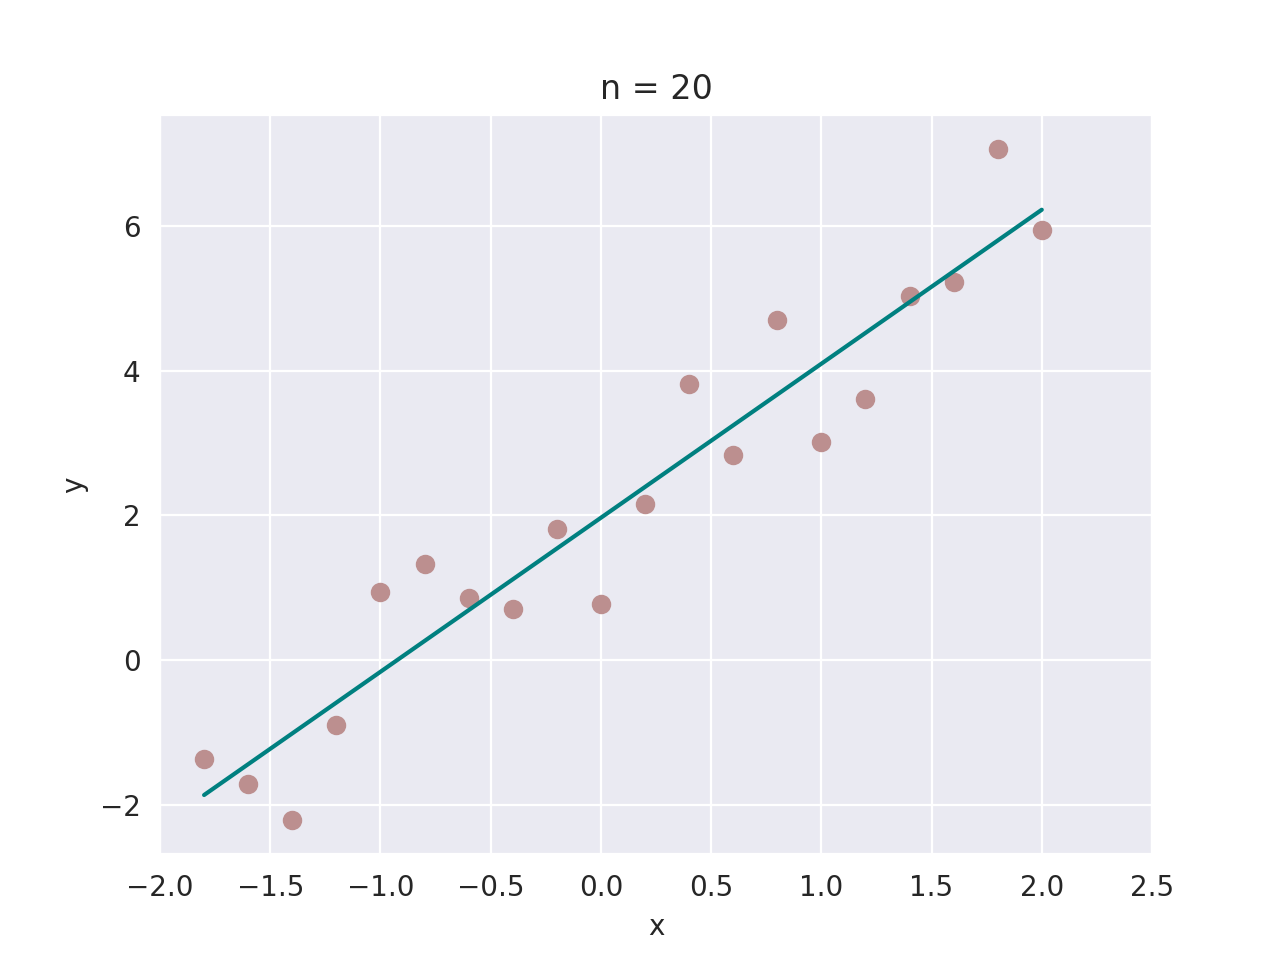
\includegraphics[width=0.5\linewidth, height=0.4\linewidth]{squares}} 
	\subfigure[]{
	\label{fig_6:2}
		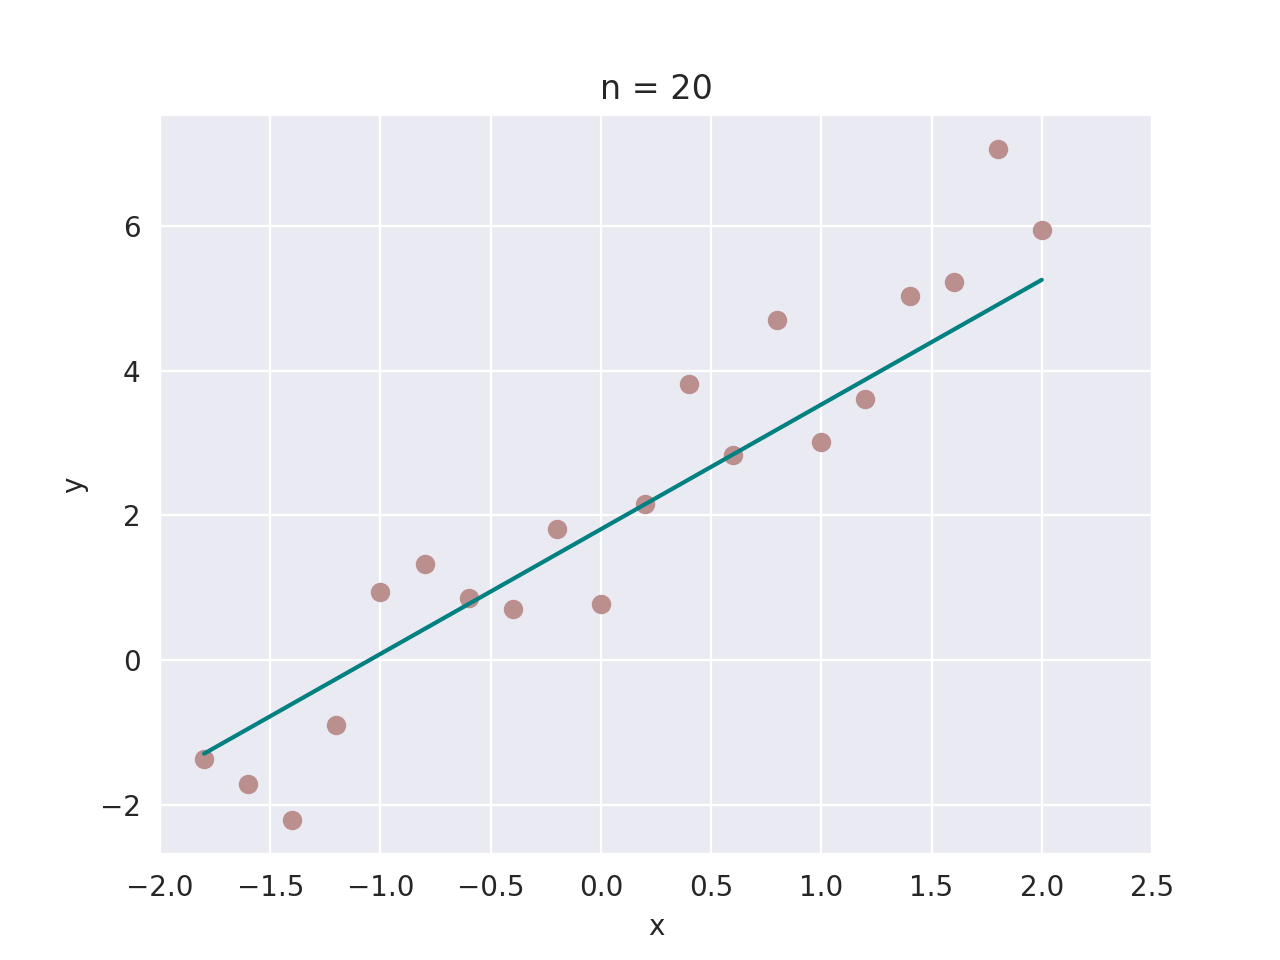
\includegraphics[width=0.5\linewidth, height=0.4\linewidth]{absolutes}}
	
	\caption{График прямой, исходные данные без возмущений
	\subref{fig_6:1} МНК; 
    \subref{fig_6:2} МНМ}
    \label{fig_6:1_2}
\end{figure}
\begin{multicols}{2}
    \raggedright
	\ref{fig_6:1}
	$\hat a = 1.9677, \; \hat b = 2.1254$

	\raggedleft
	\ref{fig_6:2}
	$\hat a = 1.8099, \; \hat b = 1.7207$
\end{multicols}
\vspace{10cm}
\begin{figure}[h!]
	\subfigure[]{
	\label{fig_6:3}
		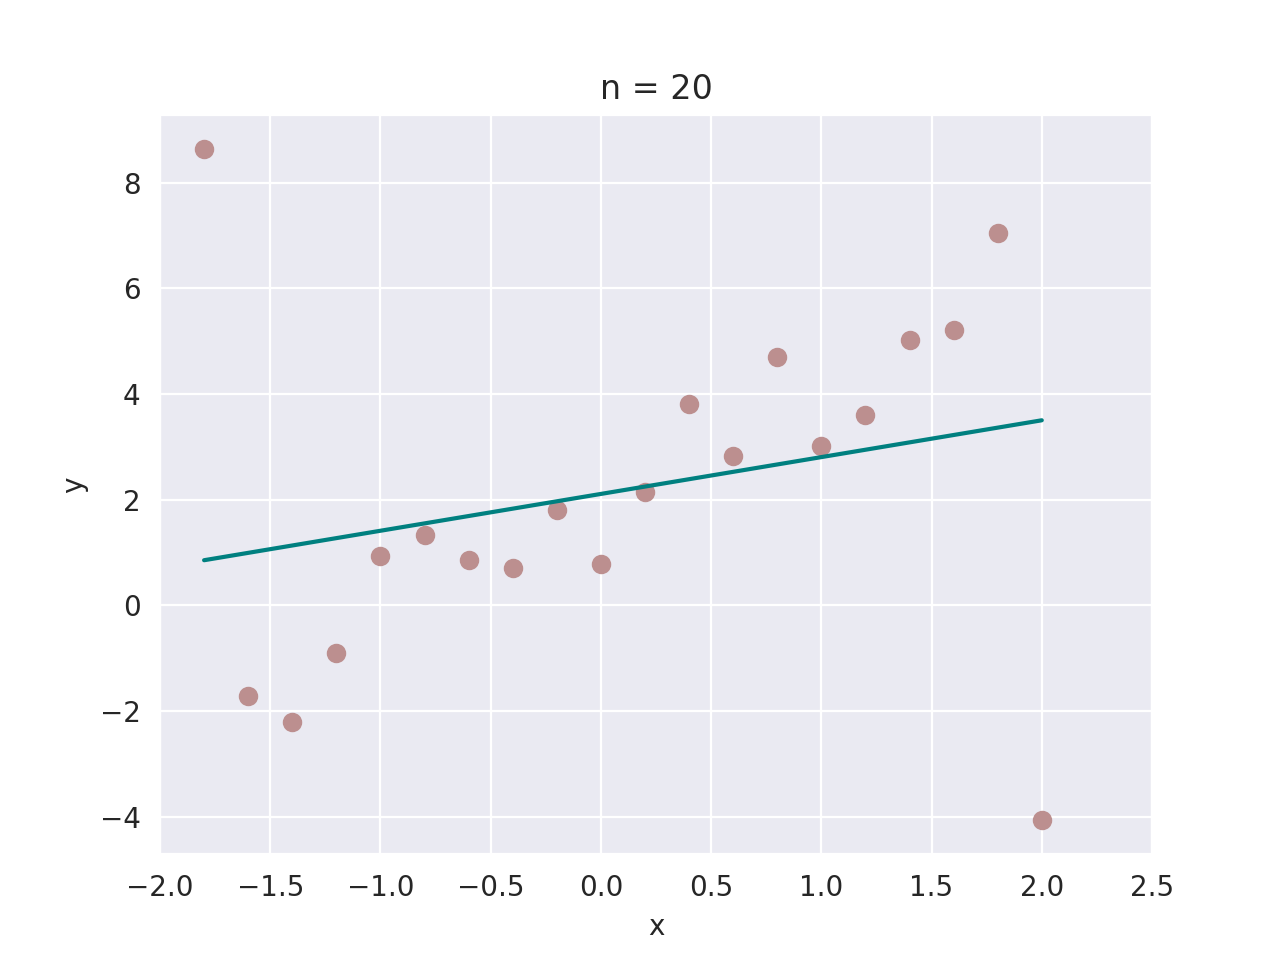
\includegraphics[width=0.5\linewidth, height=0.4\linewidth]{squares_err}} 
	\subfigure[]{
	\label{fig_6:4}
		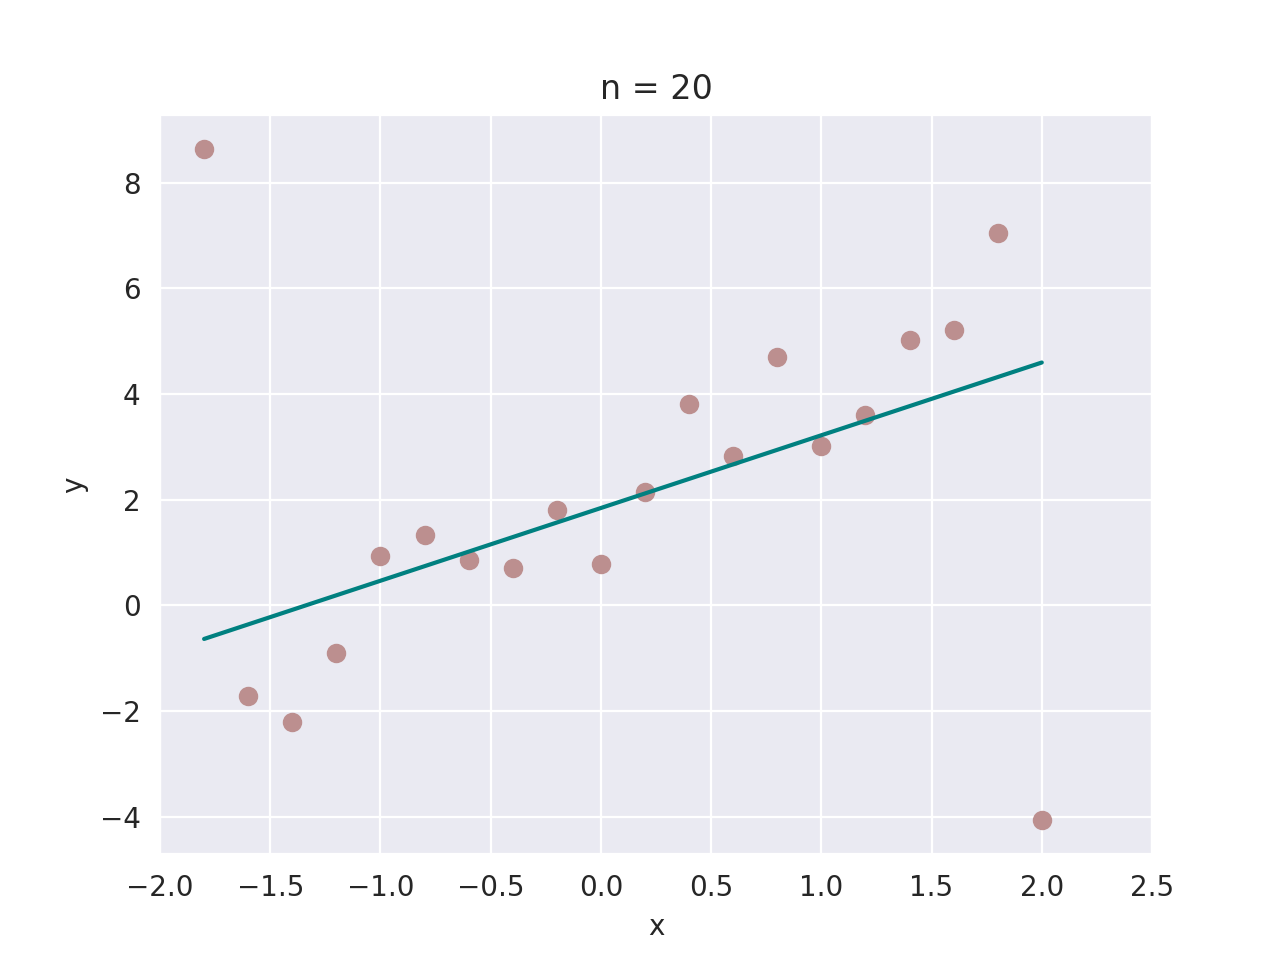
\includegraphics[width=0.5\linewidth, height=0.4\linewidth]{absolutes_err}}
	
	\caption{График прямой, исходные данные с возмущениями
	\subref{fig_6:3} МНК; 
    \subref{fig_6:4} МНМ}
    \label{fig_6:1_2}
\end{figure}
\begin{multicols}{2}
    \raggedright
	\ref{fig_6:3}
	$\hat a = 2.1106, \; \hat b = 0.6968$

	\raggedleft
	\ref{fig_6:4}
	$\hat a = 1.8443, \; \hat b = 1.3766$
\end{multicols}

\newpage
\indent{\textbf{Точечные оценки параметров}}
\begin{figure}[h!]
    \centering
    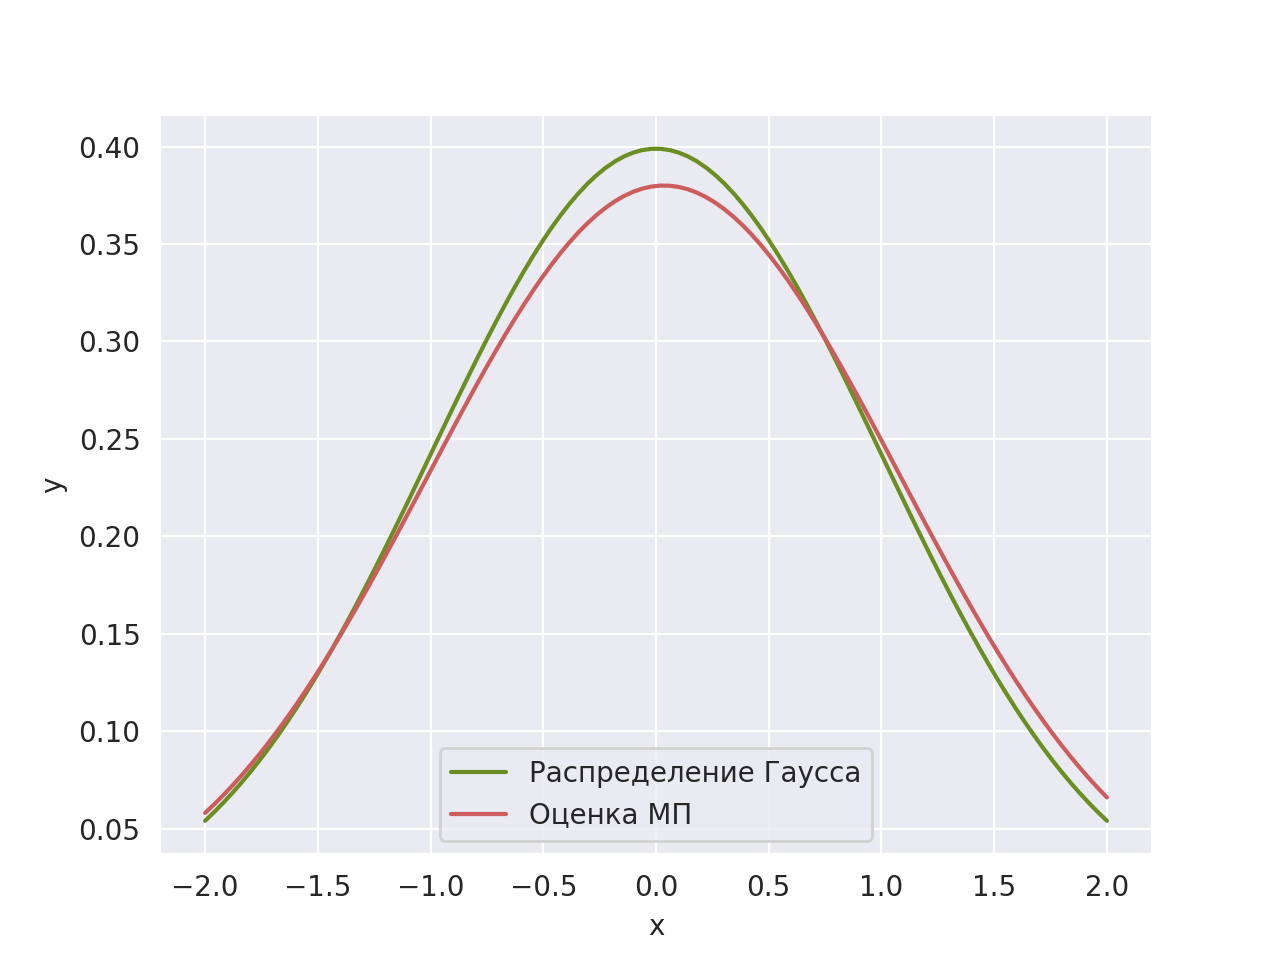
\includegraphics[width=13.5cm, height=10.cm]{mlm}
    \label{pic_7:1}
    \caption{Графики стандартного нормального распределения и распределения с параметрами, полученными методом МП}
\end{figure}
    
\newpage

\indent{Представим табулированное значение квантиля хи-квадрат, $\alpha = 0.05$}
\begin{itemize}
    \item $\chi^2_{0.95}(15) = 26.296$
\end{itemize}

\begin{center}
    \begin{tabular}{ | c | c | c | c | c | c | c | c |}
        \hline
        $k = 16$ & $a_{i - 1}$ ; $a_{i}$ & $n_i$ & $\hat p_i$ & $n_i - n \hat p_i$ & $(n_i - n \hat p_i)^2/(n \hat p_i)$ \\ \hline
        1  &  -inf ; -3.50  &  0  &  0.0004  &  -0.04  &  0.04  \\ \hline
        2  &  -3.50 ; -2.96  &  0  &  0.0018  &  -0.18  &  0.18 \\ \hline
        3  &  -2.96 ; -2.42  &  1  &  0.0074  &  0.26  &  0.09  \\ \hline
        4  &  -2.42 ; -1.88  &  2  &  0.0241  &  -0.41  &  0.07 \\ \hline
        5  &  -1.88 ; -1.35  &  3  &  0.0604  &  -3.04  &  1.53 \\ \hline
        6  &  -1.35 ; -0.81  &  14  &  0.1169  &  2.31  &  0.46 \\ \hline
        7  &  -0.81 ; -0.27  &  22  &  0.1749  &  4.51  &  1.16 \\ \hline
        8  &  -0.27 ; 0.27  &  20  &  0.2023  &  -0.23  &  0.00 \\ \hline
        9  &  0.27 ; 0.81  &  15  &  0.1809  &  -3.09  &  0.53  \\ \hline
        10  &  0.81 ; 1.35  &  11  &  0.1251  &  -1.51  &  0.18 \\ \hline
        11  &  1.35 ; 1.88  &  7  &  0.0668  &  0.32  &  0.01   \\ \hline
        12  &  1.88 ; 2.42  &  4  &  0.0276  &  1.24  &  0.56   \\ \hline
        13  &  2.42 ; 2.96  &  1  &  0.0088  &  0.12  &  0.02   \\ \hline
        14  &  2.96 ; 3.50  &  0  &  0.0022  &  -0.22  &  0.22  \\ \hline
        15  &  3.50 ; inf  &  0  &  0.0005  &  -0.05  &  0.05   \\ \hline
        $\sum$ &  –––––––– &  100  &  1  & 0 & $\chi^2_{B}$ = 5.09 \\ \hline
    \end{tabular}
    \captionof{table}{Таблица вычислений $\chi^2_{B}$ при проверке гипотезы о нормальности распределения}
\end{center}

$\chi^2_{B} = 5.09 < 26.296 \approx \chi^2_{1 - \alpha}(k - 1)$ –– гипотеза принимается

\newpage
\indent{\textbf{Интервальные оценки параметров}}

\indent{Представим значения квантилей распределений необходимых порядков, взятых из таблиц, $\alpha = 0.05$}
\begin{itemize}
    \item $t_{0.95}(19) = 1.72, \; t_{0.95}(99) = 1.66$ –– квантили распределения Стьюдента
    \item $\chi^2_{0.025}(19) = 8.91, \; \chi^2_{0.975}(19) = 32.85, \; \chi^2_{0.025}(99) = 73.12, \; \chi^2_{0.975}(99) = 128.4$ –– квантили распределения хи-квадрат
    \item $u_{0.975} = 1.96$ –– квантиль стандартного нормального распределения
\end{itemize}

\vspace{1cm}

\begin{center}
    \begin{tabular}{ | c | c | c | c |}
        \hline
        $n$ & Интервал для $\mu$ & Интервал для $\sigma$ \\ \hline
        $20$ & $(-0.239; 0.686)$ & $(0.891; 1.711)$  \\ \hline
        $100$ & $(-0.067; 0.266)$ & $(0.876; 1.160)$  \\ \hline
    \end{tabular}
    \captionof{table}{Таблица оценок на основе статистик Стьюдента и хи-квадрат}
\end{center}

\begin{center}
    \begin{tabular}{ | c | c | c | c |}
        \hline
        $n$ & Интервал для $\mu$ & Интервал для $\sigma$ \\ \hline
        $20$ & $(-0.290; 0.737)$ & $(0.873; 1.471)$  \\ \hline
        $100$ & $(-0.096; 0.295)$ & $(0.868; 1.126)$  \\ \hline
    \end{tabular}
    \captionof{table}{Таблица оценок на основе на основе асимптотического подхода}
\end{center}
\vspace{1.cm}
%%%%%%%%%%%%%%%%%%%%%%%%%%%%%%%%%%%%%%%%%%

\section*{Вывод}
\addcontentsline{toc}{section}{Вывод}

\indent{\indentРассмотрим полученные соотношения для двумерного распределения. На некоррелированных данных квадрантный коэффициент корреляции имеет наименьшую дисперсию. Также дисперсия коэффициента Пирсона всегда меньше дисперсии коэффициента Спирмена вне зависимости от объема выборки или корреляции двумерного нормального распределения \eqref{dist_5:1}. Можно полагать, что в случае такого распределения лучше рассчитывать коэффициент корреляции Пирсона.}

\indent{Неравенства для смеси двух нормальных распределений \eqref{dist_5:2} совпадают с неравенствами для двумерного нормального распределения с корреляциями $\rho = 0.5, \;0.9$.}

\indent{ Решение задачи нахождения коэффициентов линейной регрессии показало, что наиболее устойчивым критерием к выбросам является метод наименьших модулей. Выборочная медиана и интерквартильные широты менее чувствительны к выбросам, что и объясняет полученные результаты.}

\indent{ Также можно заметить, что использование метода наименьших квадратов в случае отсутствия наблюдений, не свойственных данной выборке, дает лучшие результаты. Применение МНК при наличии больших по величине выбросов имеет смысл после предварительной отбраковки значений.}

\indent{ Оценка параметров распределения методом максимума правдоподобия в случае нормального распределения  эффективна, состоятельна, асимптотически нормальна. В ходе проверки гипотезы было получено значение $\chi^2_{B} = 5.09$, являющееся очень малым, и соответствующий ему уровень значимости равен $\alpha = 0.99$, что говорит об очень хорошем согласии гипотезы $H_0$ и полученных данных.}

\indent{ По полученным интервальным оценкам можно говорить о том, что асимптотический подход не имеет преимущества по обоим параметрам сразу в случае малой выборки ($n  = 20$) при условиях, что закон распределения известен и является нормальным. При объеме выборки $n  = 100$ можно заметить сокращение длин доверительных интервалов ($0.333 < 0.391$ для $\mu$, $0.258 < 0.284$ для $\sigma$), что является преимуществом асимптотического подхода в оценке параметров распределения.}

\indent{ Недостатком интервальных оценок на основе статистик Стьюдента и хи-квадрат может выступать сложность получения точечных оценок параметра распределения, если оно не является нормальным, что в с свою очередь усложнит вычисления.}

\newpage
\begin{thebibliography}{}
    \bibitem{ms_1}\textit{Eisele, R.} (2018). How to plot a covariance error ellipse. URL: https://www.xarg.org/2018/04/how-to-plot-a-covariance-error-ellipse/
    \bibitem{ms_2}\textit{Zwillinger, D. and Kokoska, S.} (2000). CRC Standard Probability and Statistics Tables and Formulae. Chapman \& Hall: New York. 2000.
    \bibitem{ms_3}\textit{Ллойд Э., Ледерман У.} Справочник по прикладной статистике. Том 1. М.: Финансы и статистика, 1989. - 510 с.
    \bibitem{ms_4}\textit{Амосова Н.Н., Куклин Б.А., Макарова С.Б., Максимов Ю.Д., Митрофанова Н.М., Полищук В.И., Шевляков Г.Л.} Вероятностные разделы математики. Учебник для бакалавров технических направлений. –– СПб.: Иван Федоров, 2001. –– 592 с.: илл. — ISBN 5-81940-050-X.
\end{thebibliography}
\end{document}{}